\chapter{Concept}


In the last section the requirements for this project have been discussed, creating an understanding of the functional as well as nonfunctional requirements. Additionally, a way to understand the target audience using personas was prepared. \\
In this section this information will be taken to create the visual and architectural foundations of Sparked. At the end a roadmap should exist for the development process in the form of a design guide with guidelines on how to create the UI and a workflow analysis, creating an understanding which steps will be needed to meet the functional requirements as well as a shallow architectural design for the workflows specifically and the whole application in general.
\section{Visual guidelines}
Before diving into the architecture, some general guidelines for the UI should be created. These are not workflow specific but instead are mostly dependent on the target audience, which is represented by the three personas created previously: 

\begin{itemize}
\item Nora is part of the audience, viewing a Jacks presentation
\item Jack holds a presentation to demonstrate CODAs capabilities
\item Tim is a developer tasked to expand Sparked
\end{itemize}

\subsection{Looking from the users’ point of view}

\begin{description}
\item [Focus the attention.]\hfill \\
Need: Jack wants to create an order in a talk. He can not give his whole focus on the process, as he is mainly invested in relaying information to the audience. He does not want the UI to steal the focus of the audience from him, allowing him to keep Sparked open even while speaking.
Conclusion: Reduce the amount of data displayed at a given time. The user will necessarily be focused on a specific item if it is the only one on the screen. Hiding or graying out other elements will be used if possible.
Similarly having long lists with many items holds the focus of the viewer for a long time. Reducing the number of items visible at any given time, using bigger fonts will reduce the time the viewer needs to take their focus back to the presentation, even if this means that the information density is reduced, and more scrolling is needed. 
\item [Good readability.]\hfill \\
Need: As a viewer of the presentation Nora wants to be able to follow what is visible on the screen, even if lighting is not favorable or she is sitting on the far end. 
Conclusion: A high contrast color scheme should help readability. Using bigger fonts and lines with higher thickness will help as well. 
\end{description}

With these requirements in mind a set of design goals can be formulated.
\begin{itemize}
\item \textbf{Reduce the information density}
\end{itemize}
In many UIs the goal is, to put as much information and functionality into as little space as possible. A good example of this trend is the UI of OpenML, where the font becomes small and data points are only separated by a dash, not by a visual element. On a computer screen this will allow a user to see most relevant data without switching in and out of detail pages, reducing the amounts of mouse interactions they must do. On a beamer could easily become a distraction, taking the focus of the audience away from the presentation while they are trying to decipher the small fonts. 
\begin{itemize}
\item \textbf{High contrast, big font}
\end{itemize}
This too is a way to make the UI as readable as possible. Especially if the UI is displayed on a beamer, this becomes important, as lighting conditions are often not optimal.
\begin{itemize}
\item \textbf{Use a strong color to guide the attention}
\end{itemize}
Color is a good way to grab the attention of the viewer. Having a selected item light up with a strong color can be used like a flashlight to indicate the important pieces of information. Trouble arises, when too much color is used. If several pieces are strongly colored, it loses its potency to grab the attention. 
\begin{itemize}
\item \textbf{Use the same look and feel throughout the application}
\end{itemize}
Using the same places for related purposes on all views and reusing visual elements in the entire application and using uniform font and color scheme, allows the user to become familiar with the UI faster, which is in most cases wanted by the designer. \\
The first step in creating a common look and feel is to create a common map of where what kind of information goes on the screen. The first concern is to keep the UI close to what the user would expect, which means putting the icon in the top left corner and title information close to the top. \\
For this design the center will be used for main information, like the list of orders or the diagrams for the evaluation view. On the left side, functions like ok and cancel will be situated Whereas information text, that may describe certain functions or data will be on the right. 

\begin{figure}
	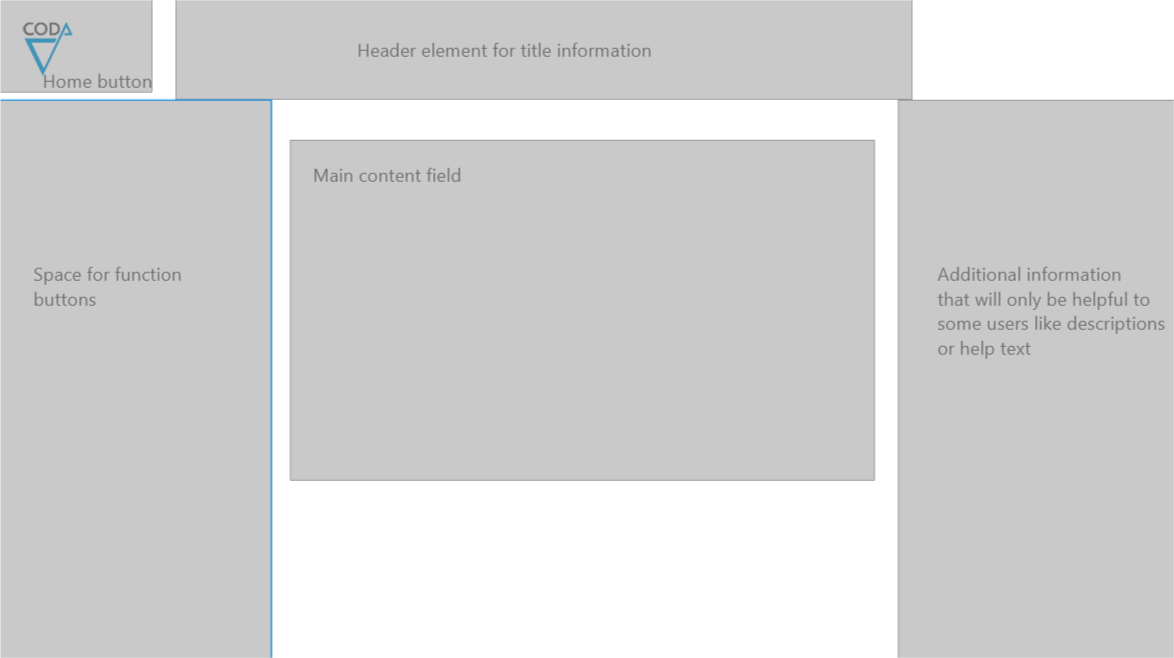
\includegraphics[width=\textwidth]{BasicLayout.png}
	\caption{Segmenting the UI}
\end{figure} 

\section{Architecture}
Armed with an understanding of what Sparked is set out to accomplish, a rough architecture will be created. Software architecture is a very wide field that may be used to define a program down to a level only just above the implementation itself. For this project a rough overview of the components however should be enough. Creating detailed UML (Unified Modeling Language) descriptions of an application is very time consuming and it always needs to be calculated whether the development speed or code quality gained is worth the amount of work put into documenting an architecture beforehand. 

\subsection{The 30000-foot view}
To start with it is helpful to view the whole project from a distance. Creating a first high level architectural description, often called the 30000-foot view, will help assess the core concepts and major building blocks.
 
\begin{figure}
	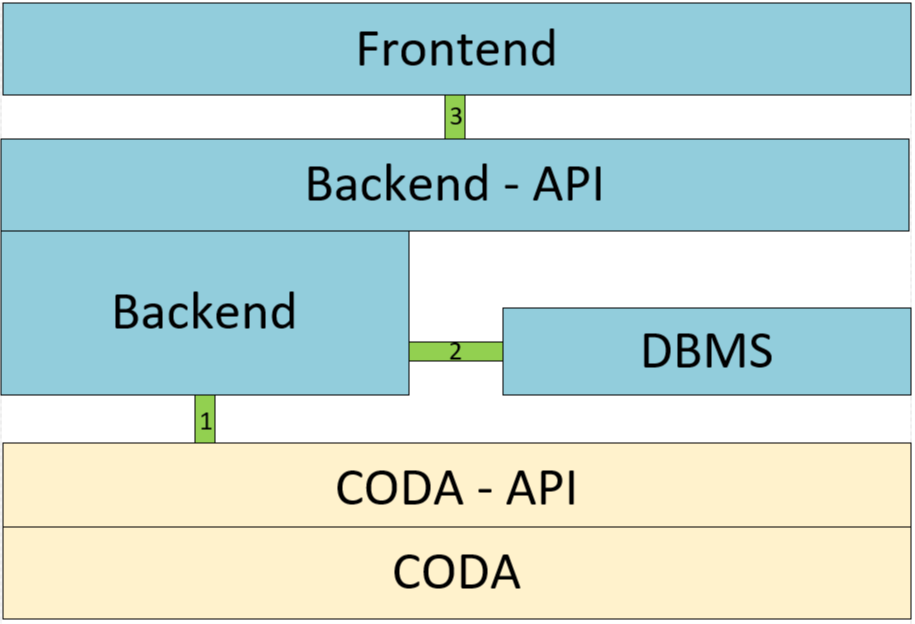
\includegraphics[width=\textwidth]{30000-foot.png}
	\caption{30000-foot view of Sparked architecture }
\end{figure}

In this diagram yellow parts are provided. White space indicates the possibility to distribute parts on different systems. Green lines show points of interaction between the different parts.
A point of interest is the CODA API and the interaction line 1, since this is the part that is defined outside of Sparked. This means, that the technology and structure are already known. The API itself is a REST API, using JSON (JavaScript Object Notation) for data transfer. Its endpoints deliver the building blocks of all further development. 
There are four endpoints delivering the supported classifiers, validation methods, datasets and evaluation metrics. An endpoint with the status of all orders, one to get the status of a specific order and one to get the results for a specific order and an endpoint each to start a task or an order. [For a more comprehensive description see the API description by the CODA team, listing 1 and 2\\ XXXXXXXXXXXXXXXXXXXXXXXXXXXXXXXXXXXXXXXXXXXXXXXXXXXXXXXXXXXXXXXXXXXXXXXXXXXXXXXXXXXXXXXXXXXXXXXXXXXXXX link to Coda api chapter \\
It is to note that CODA is still in development, therefore the API might be subject to change in the future. 

\subsection{Workflows}
Having defined the central building blocks, it is now time to look at the workflows needed to satisfy the functional requirements. To recap, the functional requirements for Sparked are:
\begin{itemize}
\item Creating an order
\item Starting an order
\item Listing existing orders
\item Displaying the evaluation data of a completed order
\end{itemize}

\subsubsection{Workflow: Create and start an order}
An order is a set of tasks, that only differs in the classifier, while a task combines all information needed to run an evaluation. That an order may not contain tasks differing in features other than the classifier is not inherent to the concept of an order. As such this boundary condition will not be put into the basic structure, making it easier to change in future. 
The final feature of an order is a status information, reflecting whether the order is new, has been started, completed or if an error has occurred.
 
\begin{figure}
	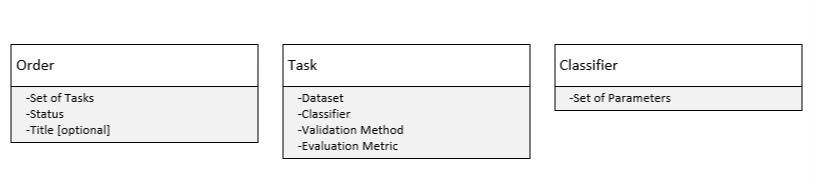
\includegraphics[width=\textwidth]{Order-BasicModel.png}
	\caption{Data needed to define an Order}
\end{figure}

An activity diagram of the order creation workflow for a better overview. Creating it helps to get into the mindset of what the workflow entails. Later in development it can be used as a red line on what needs to be done.
 
\begin{figure}
	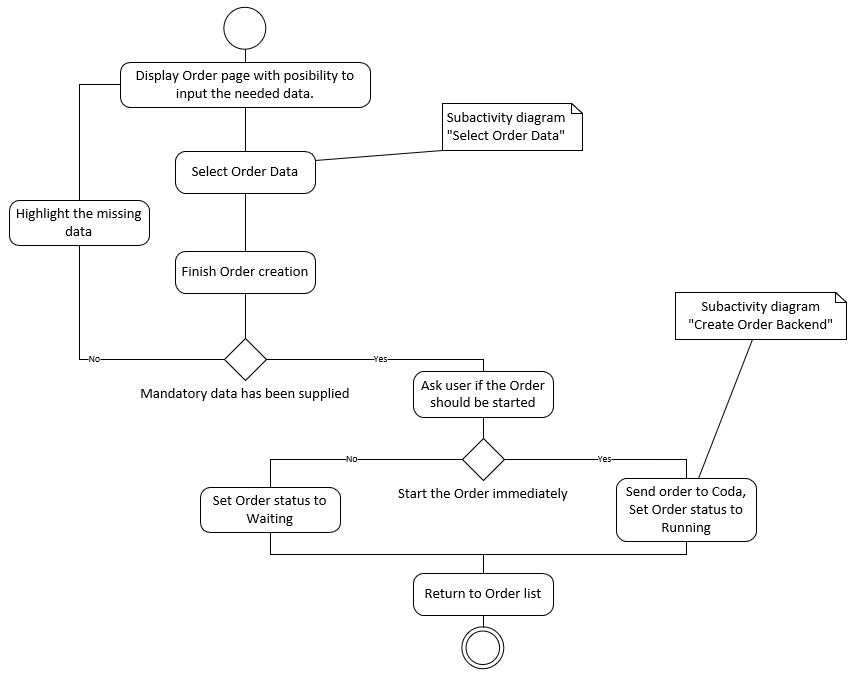
\includegraphics[width=\textwidth]{AD-CreateOrder.png}
	\caption{Activity Diagram – Create Order}
\end{figure}

From the activity diagram four parts can be identified.
\begin{itemize} 
\item The data input or selection
\item Create the Order and validate whether necessary data has been supplied
\item Check if Order should be started immediately
\item Start the order
\end{itemize}

One of the mayor scenarios is to show example orders in a presentation or similar format. Creating and starting an order from scratch in such a situation has the problem, that the runtime for machine learning tasks can be quite substantial. This would mean finding the correct order out of a possible longer list in a short amount of time. To support this, it would be helpful for the user to give a kind of identity to an order. \\
Since Sparked has its own data storage, it is possible to add additional data to an order, that is not supported by CODA itself. For this scenario it was decided, to have an additional optional title field. This does not change the fundamental workflow, only adds an additional step in selecting the order data, but also shows a way for future expansion. If ever concepts like labeling of orders or user accounts may become relevant, they can be achieved with the same concept as the title field.

\subsubsection{Workflow: Listing orders}
Once orders can be created, showing and opening all existing orders becomes the next workflow to consider. 
Its main goal of this workflow is:

\begin{itemize}
\item See all orders created by this instance of Sparked and to 
\item Open detail page of a single order
\item Open evaluation page of completed evaluations and display the evaluation data returned by CODA
\end{itemize}

The first part is rather straight forward from a UI point of view. Get a list of orders and display some of its data in a table like view. 
There are two points to consider:\\
The first is, that the status information of an order is an important information in this list. The status is however subject to change and its current value can only be supplied by the CODA backend. This means a UI request to display the order list must receive data not only from Sparked but from CODA as well. This has the potential to be slow and must be considered when implementing. \\
A way around would be by loading the data beforehand in an asynchronous manner. Ideally this would be done by having the CODA API push the data or a data changed information towards Sparked whenever a status has changed. The CODA API does not allow for this though, making a polling approach the only viable option for preloading. Since the data will contain information on all orders this may in future become a large and costly request. At the same time the information should not become too old as for the user to wait on an order that has already been finished. As a good polling timer is rather subjective this is a time a value should be changeable via the application properties.\\
The second problem is on which orders to show. Both the CODA API as well as Sparks own database may contain orders, but an order that was never started will only appear on the internal database, while an order that was started with for example a different Sparked instance, will only be available via the CODA API. \\
One of the starting requirements is, that Sparked must support a clean slate startup. Since deleting orders via the CODA API is not possible and probably not wanted, the decision was made, to only show orders that have a corresponding entry in the applications own database. 

\subsubsection{Workflow: Evaluation}
The last workflow is the evaluation. Here an order is open XXXXXXXXXXXXXXX

